\section{Efficient Enumeration of Ladder Lotteries and its Application}

%%Intro
In \emph{Efficient Enumeration of Ladder Lotteries and its Application}~\cite{A1}, written by Yamanaka, Nakano, Matsui, Uehara, and Nakada, 
the authors provide an algorithm for generating $OptL\{\pi\}$ 
for any $\pi$, in $\mathcal{O}(1)$ time per ladder. The authors refer to this algorithm as {\sc FindAllChildren}.




%%Put this in the Appendix

%%DONE PUT IN Appendix

%%%%%%%%%%%%%%%%%%%%%%%%%%%%%%%FIND ALL CHILDREN ALGORITHM%%%%%%%%%%%%%%%%%%%%%%%%%%%%%



%%%%%%%%%%%%%%%%%%END ALGORITHM%%%%%%%%%%%%%%%%%%%%%%%%%%



{\sc FindAllChildren} was used in this thesis to generate the sample data that aided in finding solutions for 
the Canonical Ladder Listing Problem.
To see the tree structure generated by {\sc FindAllChildren} for $OptL\{(4,3,2,1)\}$ 
please refer to Figure~\ref{Fig:TreeFAC}.\par
\begin{figure}[h]
	\centering 
	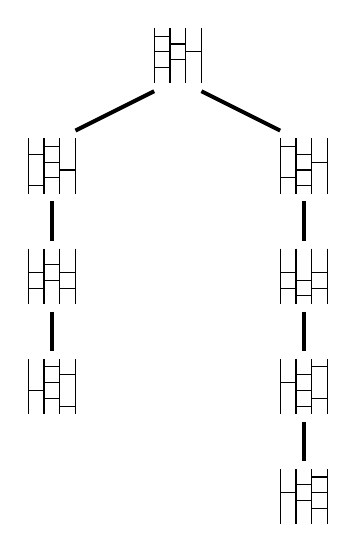
\begin{tikzpicture}
		%%L1
		\draw(5, 10) to (5, 9.3);
			\draw(5, 9.9) to (5.2, 9.9);
			\draw(5.2, 9.8) to (5.4, 9.8);
			\draw(5.4, 9.7) to (5.6, 9.7);
		\draw(5.2, 10) to (5.2, 9.3);
			\draw(5, 9.7) to (5.2, 9.7);
			\draw(5.2, 9.6) to (5.4, 9.6);
		\draw(5.4, 10) to (5.4, 9.3);
			\draw(5, 9.5) to (5.2, 9.5);
		\draw(5.6, 10) to (5.6, 9.3);
		%L2
		\draw[line width = .5mm](5, 9.2) to (4, 8.7);
		\draw[line width = .5mm](5.6, 9.2) to (6.6, 8.7);
			%%L2
			\draw(3.4, 8.6) to (3.4, 7.9);
				\draw(3.4, 8.4) to (3.6, 8.4);
				\draw(3.4, 8) to (3.6, 8);
			\draw(3.6, 8.6) to (3.6, 7.9);
				\draw(3.6, 8.5) to (3.8, 8.5);
				\draw(3.6, 8.3) to (3.8, 8.3);
				\draw(3.6, 8.1) to (3.8, 8.1);
			\draw(3.8, 8.6) to (3.8, 7.9);
				\draw(3.8, 8.2) to (4, 8.2);
			\draw(4.0, 8.6) to (4.0, 7.9);

				%%level
				\draw[line width = .5mm](3.7, 7.8) to (3.7, 7.3);
			\draw(3.4, 7.2) to (3.4, 6.5);
				\draw(3.4, 6.9) to (3.6, 6.9);
				\draw(3.4, 6.7) to (3.6, 6.7);
			\draw(3.6, 7.2) to (3.6, 6.5);
				\draw(3.6, 7) to (3.8, 7);
				\draw(3.6, 6.8) to (3.8, 6.8);
			\draw(3.8, 7.2) to (3.8, 6.5);
				\draw(3.8, 6.9) to (4, 6.9);
				\draw(3.8, 6.7) to (4, 6.7);
			\draw(4.0, 7.2) to (4.0, 6.5);

		%%L3
			\draw(6.6, 8.6) to (6.6, 7.9);
				\draw(6.6, 8.5) to (6.8, 8.5);
				\draw(6.8, 8.4) to (7, 8.4);
				\draw(7, 8.3) to (7.2, 8.3);
			\draw(6.8, 8.6) to (6.8, 7.9);
				\draw(6.8, 8.2) to (7, 8.2);
				\draw(6.8, 8) to (7, 8);
			\draw(7, 8.6) to (7, 7.9);
				\draw(6.6, 8.1) to (6.8, 8.1);
			\draw(7.2, 8.6) to (7.2, 7.9);
			
			
			\draw[line width = .5mm](6.9, 7.8) to (6.9, 7.3);

			\draw(6.6, 7.2) to (6.6, 6.5);
				\draw(6.6, 6.9) to (6.8, 6.9);
				\draw(6.6, 6.7) to (6.8, 6.7);
			\draw(6.8, 7.2) to (6.8, 6.5);
				\draw(6.8, 6.8) to (7, 6.8);
				\draw(6.8, 6.6) to (7, 6.6);
			\draw(7.0, 7.2) to (7.0, 6.5);
				\draw(7, 6.9) to (7.2, 6.9);
				\draw(7, 6.7) to (7.2, 6.7);
			\draw(7.2, 7.2) to (7.2, 6.5);

			\draw[line width = .5mm](3.7, 6.4) to (3.7, 5.9);

			\draw(3.4, 5.8) to (3.4, 5.1);
				\draw(3.4, 5.4) to (3.6, 5.4);
			\draw(3.6, 5.8) to (3.6, 5.1);
				\draw(3.6, 5.7) to (3.8, 5.7);

				\draw(3.6, 5.5) to (3.8, 5.5);
				\draw(3.6, 5.3) to (3.8, 5.3);
			\draw(3.8, 5.8) to (3.8, 5.1);
				\draw(3.8, 5.6) to (4, 5.6);
				\draw(3.8, 5.2) to (4, 5.2);
			\draw(4.0, 5.8) to (4.0, 5.1);

			\draw[line width = .5mm](6.9, 6.4) to (6.9, 5.9);

			
			\draw(6.6, 5.8) to (6.6, 5.1);
				\draw(6.6, 5.5) to (6.8, 5.5);
			\draw(6.8, 5.8) to (6.8, 5.1);
				\draw(6.8, 5.6) to (7, 5.6);

				\draw(6.8, 5.4) to (7, 5.4);
				\draw(6.8, 5.2) to (7, 5.2);
			\draw(7.0, 5.8) to (7.0, 5.1);
				\draw(7.0, 5.7) to (7.2, 5.7);
				\draw(7.0, 5.3) to (7.2, 5.3);
			\draw(7.2, 5.8) to (7.2, 5.1);

			\draw[line width = .5mm](6.9, 5) to (6.9, 4.5);

			\draw(6.6, 4.4) to (6.6, 3.7);
				\draw(6.6, 4.1) to (6.8, 4.1);
			\draw(6.8, 4.4) to (6.8, 3.7);
				\draw(6.8, 4.2) to (7, 4.2);

				\draw(6.8, 4) to (7, 4);
			\draw(7.0, 4.4) to (7.0, 3.7);
				\draw(7.0, 4.3) to (7.2, 4.3);
				\draw(7.0, 4.1) to (7.2, 4.1);
				\draw(7.0, 3.9) to (7.2, 3.9);
			\draw(7.2, 4.4) to (7.2, 3.7);



	\end{tikzpicture}
	\caption{The tree structure of $OptL\{(4,3,2,1)\}$ generated by {\sc FindAllChildren}}
	\label{Fig:TreeFAC}
\end{figure}
\pagebreak
Let $x>y>z$ be any three elements in $\pi$. We define 
$pos(x)$ as the position of $x$ in $\pi$.
Let $pos(x) < pos(z)$ and let $pos(y) < pos(z)$. 
Let $l$ be a ladder lottery in $OptL\{\pi\}$. 
Let $(x,z)$ be a bar in $l$ where $x$ and $z$ interchange. Let $(y,z)$ 
be a bar in $l$. We say the \emph{clean level} of $l$ is $1$ 
plus the maximum value of $x$ for which the following property holds: $\exists (x,z) \text{ below } (y,z) \in l$. 
Then, we say the clean level is $x+1$. If no such $x$ exists, we say the clean level of a ladder is $1$. 
Yamanaka, Nakano, Matsui, Uehara, and Nakada show that the ladder with a clean level of $1$ is unique in $OptL\{\pi\}$. This ladder 
is known as the \emph{root ladder}. The authors do not provide an algorithm for creating the root ladder. 
The algorithm {\sc CreateCanonical} found in Chapter 3 creates the root ladder for $OptL\{\pi\}$. 
Hence, we provide the algorithm for creating the root ladder.
To see the root ladder of $OptL\{(4,5,6,3,1,2)\}$ please refer to Figure~\ref{fig:root}, which we note has a clean level of $1$.  

%%%%%%%%%%%%%ROOT LADDER FIGURE%%%%%%%%%%%%%%%%%%%%%%%
\begin{figure}[h]


	\begin{center}
		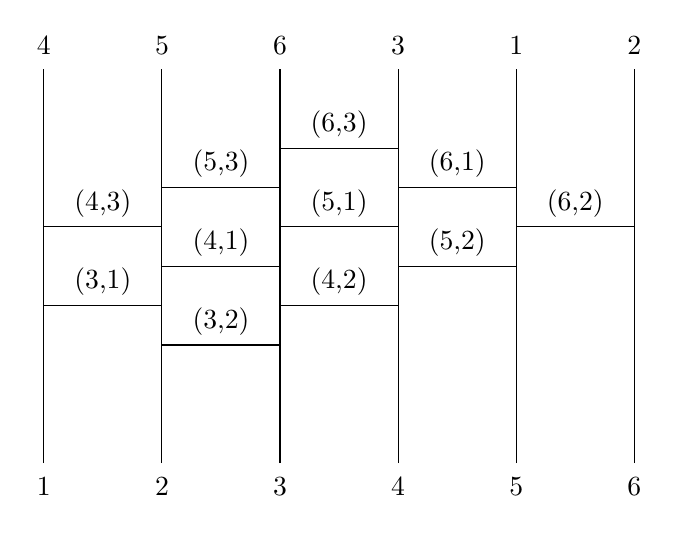
\begin{tikzpicture}
			%%draw the lines
			\draw(0, 0) to (0, 5);
				\node at (0, 5.3){4};
				\node at (0, -0.3){1};

			\draw(1.5, 0) to (1.5, 5);
				\node at (1.5, 5.3){5};
				\node at (1.5, -0.3){2};
			
			\draw(3, 0) to (3, 5);
				\node at (3, 5.3){6};
				\node at (3, -0.3){3};
			\draw(4.5, 0) to (4.5, 5);
				\node at (4.5, 5.3){3};
				\node at (4.5, -0.3){4};
			\draw(6, 0) to (6, 5);
				\node at (6, 5.3){1};
				\node at (6, -0.3){5};
			\draw(7.5, 0) to (7.5, 5);
				\node at (7.5, 5.3){2};
				\node at (7.5, -0.3){6};

			%%draw the bars
			
			%%6's route
			\draw(3, 4) to (4.5, 4);
				\node at (3.75, 4.3){(6,3)};
			\draw(4.5, 3.5) to (6, 3.5);
				\node at (5.25, 3.8){(6,1)};
			\draw(6, 3) to (7.5, 3);
				\node at (6.75, 3.3){(6,2)};
			%%5's route
			\draw(1.5, 3.5) to (3, 3.5);
				\node at (2.25, 3.8){(5,3)};
			\draw(3, 3) to (4.5, 3);
				\node at (3.75, 3.3){(5,1)};
			\draw(4.5, 2.5) to (6, 2.5);
				\node at (5.25, 2.8){(5,2)};
			%draw 4's route
			\draw(0, 3) to (1.5, 3);
				\node at (0.75, 3.3){(4,3)};
			\draw(1.5, 2.5) to (3, 2.5);
				\node at (2.25, 2.8){(4,1)};
			\draw(3, 2) to (4.5, 2);
				\node at (3.75,2.3){(4,2)};

			%%draw 3's route
			\draw(0, 2) to (1.5, 2);
				\node at (0.75, 2.3){(3,1)};
			\draw(1.5, 1.5) to (3, 1.5);
				\node at (2.25, 1.8){(3,2)};
		\end{tikzpicture}

	\end{center}





	\caption{The root ladder for $OptL\{(4,5,6,3,1,2)\}$. Notice how the clean 
	level of this ladder is $1$, thus making it the root ladder.} 
	\label{fig:root}

\end{figure}





%%Root ladder subsection




%%DONE Appendix SECTION


